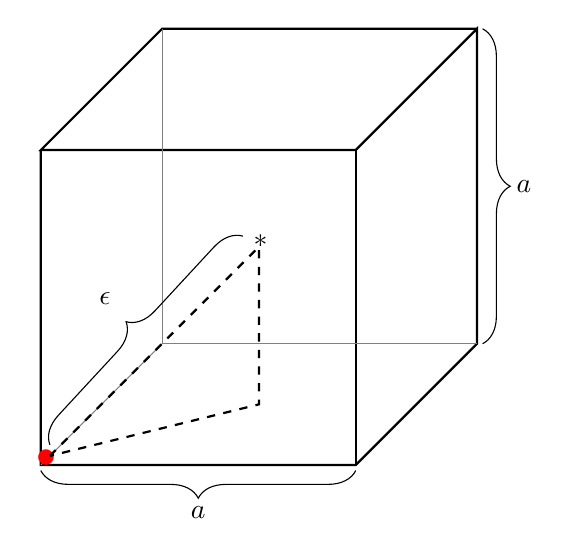
\begin{tikzpicture}
    \draw[thick](4,4,0)--(0,4,0)--(0,4,4)--(4,4,4)--(4,4,0)--(4,0,0)--(4,0,4)--(0,0,4)--(0,4,4);
    \draw[thick](4,4,4)--(4,0,4);
    \draw[gray](4,0,0)--(0,0,0)--(0,4,0);
    \draw[gray](0,0,0)--(0,0,4);
    
    \draw(0,0,3.8) node{\Large\textcolor{red}{$\bullet$}};
    \draw[dashed, thick](0,0,3.7) -- (2,2,2) -- (2,0,2) -- (0,0,3.7);
    \draw(2,2.05,1.95) node{$\mathbf{\ast}$};
  
  \draw [decorate,decoration={brace,amplitude=10pt},xshift=-0pt,yshift=4pt]
  (0,0,3.7) -- (1.8,2,2)node [black,midway,yshift=15pt,xshift=-15pt] {$\epsilon$};  
  \draw [decorate,decoration={brace,amplitude=10pt, mirror},xshift=0pt,yshift=-2pt]
  (0,0,4) -- (4,0,4)node [black,midway,yshift=-15pt] {$a$};
  \draw [decorate,decoration={brace,amplitude=10pt},xshift=2pt,yshift=0pt]
  (4,4,0) -- (4,0,0)node [black,midway,xshift=15pt] {$a$};
  \end{tikzpicture}